\section{Introduction}
Recent advances in spoken dialogue systems have shifted from turn-based, half-duplex models to full-duplex systems capable of simultaneous listening and speaking \citep{arxiv:2503.01174, dgslm,vap}. Under this setting, the dominant paradigms frame this task as prediction. The first approach, Next Segment Prediction, models the agent's response as a complete turn \citep{hara18_interspeech, li-etal-2022-speak, 5494991}. A more recent approach, Next Dual-Token Prediction, generates simultaneous token streams for both speakers to better handle overlap and real-time interaction \citep{arxiv:2203.16502, defossez2024moshi}. While these methods have improved system responsiveness, they treat conversation as a sequence generation problem, bypassing the cognitive layer of reasoning that governs human interaction \citep{monroe2015learningrationalspeechacts,zhixuan2024pragmaticinstructionfollowinggoal}.

Human conversation, however, operates on a more abstract and causal level. When Speaker 1 produces an utterance, Speaker 2 does not simply predict the next sequence of words. Instead, they first perceive the behavior (e.g., recognizing a constative speech act), which triggers an internal chain of thought (e.g., deciding not to interrupt and to remain silent). This reasoning process culminates in a generated action (e.g., an acknowledgement). This gap between pattern matching and causal reasoning is a fundamental barrier to creating truly natural AI agents. Meanwhile, full-duplex interaction imposes strict real-time requirements. When an agent is listening and speaking at the same time, it must make decisions at a per-second granularity; consequently, latency must be upper-bounded and throughput must remain stable. Our work addresses the core scientific question: under the full-duplex task setting, how can a machine model this perception-reasoning-generation loop to make principled, interpretable decisions in real time?

\begin{figure*}[t]
    \centering
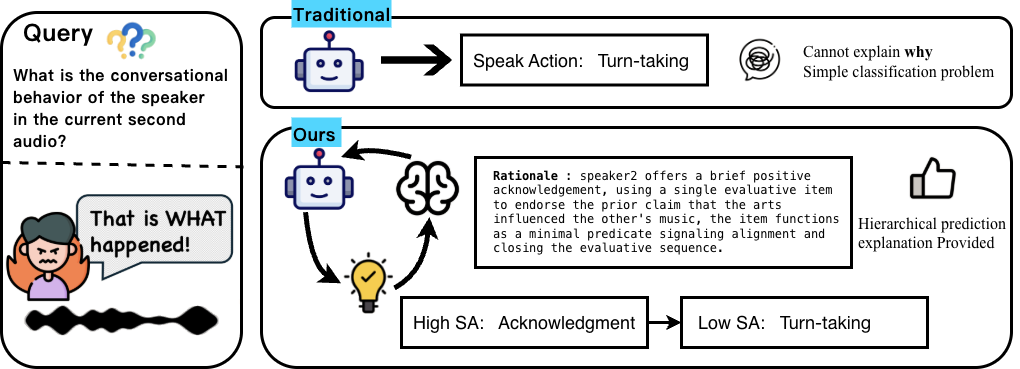
\includegraphics[width=0.9\linewidth]{fig/intro/framework_2.png}
\vspace{-5pt}
    \caption{{\bf Comparison of dialogue paradigms.} (Traditional) Traditional duplex systems frame conversation as a direct sequence prediction task. (Ours) We propose a framework based on next-behavior perception and reasoning: the agent first perceives the speaker’s behaviors at multiple levels, then reasons via a Graph-of-Thoughts, and finally generates a response.}
    \label{demo-fig-main}
\end{figure*}

To tackle this challenge, we introduce a framework that operationalizes the process. Our approach is twofold. First, we formalize the Perception stage with a hierarchical conversational behavior detection model. This module learns to identify conversational behaviors at two dimensions. It first captures high-level speech acts (e.g., {\em constative, directive}) \citep{jurafsky2025speech} that reflect coarse-grained communicative intent. Then, guided by these high-level acts, it predicts low-level interaction behaviors (e.g., {\em turn-taking, backchannel}) that describe interaction mechanics \citep{schegloff1982discourse, gravano2011turn, duncan1972some, raux2012optimizing, khouzaimi2016reinforcement, marge2022spoken, arxiv:2503.04721, arxiv:2503.01174, dgslm}. This provides the system with a structured understanding of the ongoing dialogue. Second, we model the explicit reasoning process with a Graph-of-Thoughts (GoT) system \citep{got}. The system constructs a causally inspired dynamic graph from the sequence of perceived speech acts, capturing the evolving chain of thoughts within the conversation. By performing inference over this graph, our model can not only predict the most appropriate subsequent behavior, but also generate a natural language rationale explaining its decision. This transforms the opaque prediction task into an auditable reasoning process, which provides a unified benchmark for \textit{evaluating conversational behavior in duplex speech systems.}

To train this framework, we construct a high-quality hybrid corpus that combines behavior-rich simulated dialogues with high-quality synthetic annotations that are manually verified. Models trained on this corpus generalize well when transferred to real-world conversational datasets with substantially different discourse distributions. This indicates that our synthetic data effectively reproduces key interactional structures of human conversation (e.g., turn-taking dynamics), while the introduced annotations provide a high-fidelity characterization of conversational behaviors and the rationales underlying them.


In summary, our contributions are:
{%
\setlength{\topsep}{0pt}
\setlength{\itemsep}{0pt}
\setlength{\parskip}{0pt}
\setlength{\parsep}{0pt}
\setlength{\partopsep}{0pt} 
\begin{itemize}
    \item A conceptual shift from next-token prediction to next-behavior reasoning for full-duplex interaction, demonstrating that modeling the causal chain from intent to action is essential for natural dialogue.
    
    \item A hierarchical speech act detection model that perceives conversational behaviors at both high (intent) and low (action) levels, serving as a foundational module for reasoning-driven dialogue systems.
    
    \item A GoT framework for conversational reasoning that models intent-act dynamics as a causal graph, enabling real-time, interpretable decision-making and rationale generation.
    
    \item A comprehensive empirical validation demonstrating that our system effectively detects conversational behaviors, generates plausible rationales, and successfully transfers its reasoning capabilities from simulated to real-world full-duplex systems.
\end{itemize}
}%
